
\section*{Постановка задачи}
Необходимо разработать универсальный класс для хранения данных в виде хеш-таблицы.

Универсальный класс хеш-таблица может иметь тип <$K$, $V$>, где $K$ - ключ, а $V$ - значение.

Класс должен быть сериализуемым, то есть его можно было бы конвертировать в \textit{JSON} или \textit{XML} формат, а так же десериализуемым, чтобы можно из файла создавать структуру данных во время исполнения программы.

Проект должен иметь тесты, графический интерфейс, консольное приложение и саму библиотеку.
\addcontentsline{toc}{section}{Постановка задачи}

\newpage
\section{Введение}

В компьютерных науках \textbf{хеш-таблица} (также можно использовать слово хэш) (\textbf{hash-map}) представляет собой структуру данных, которая реализует абстрактный тип данных ассоциативного массива, структуру, которого является сопоставлением ключей с значением.
Хеш-таблица использует хэш-функцию для вычисления индекса, также называемого \textit{хэш-кодом}, в массиве \textit{сегментов} (\textit{buckets}) или \textit{слотов}, из которых можно получить желаемое значение. 
Во время поиска ключ хэшируется, и результирующий хэш указывает, где хранится соответствующее значение.

В идеале хэш-функция будет назначать каждый ключ уникальному сегменту, но в большинстве конструкций хэш-таблиц используется несовершенная хэш-функция, которая может привести к \textit{коллизии} хешей, которое происходит, когда хэш-функция генерирует один и тот же индекс для более чем одного ключа. 
Такие коллизии обычно каким-то образом разрешаются.

В хэш-таблице с некими размерами средняя стоимость (количество инструкций) для каждого поиска не зависит от количества элементов, хранящихся в таблице.
Многие конструкции хэш–таблиц также допускают произвольные вставки и удаление пар ключ-значение при постоянной (амортизированной) средней стоимости за операцию.

Хеширование - это пример компромисса между пространством и временем. 
Если память бесконечна, все ключи можно использовать непосредственно в качестве индекса для определения его значения с помощью одного прямого доступа к месту памяти элемента. 
С другой стороны, если время бесконечно, значения могут храниться без учета их ключей, и двоичный поиск или линейный поиск могут быть использованы для извлечения элемента.

Во многих ситуациях хэш-таблицы оказываются в среднем более эффективными, чем деревья поиска или любая другая структура поиска по таблицам. 
По этой причине они широко используются во многих видах компьютерного программного обеспечения, особенно для ассоциативных массивов, индексации баз данных, кэшей и множеств.

\begin{figure}[H]
	\begin{center}
		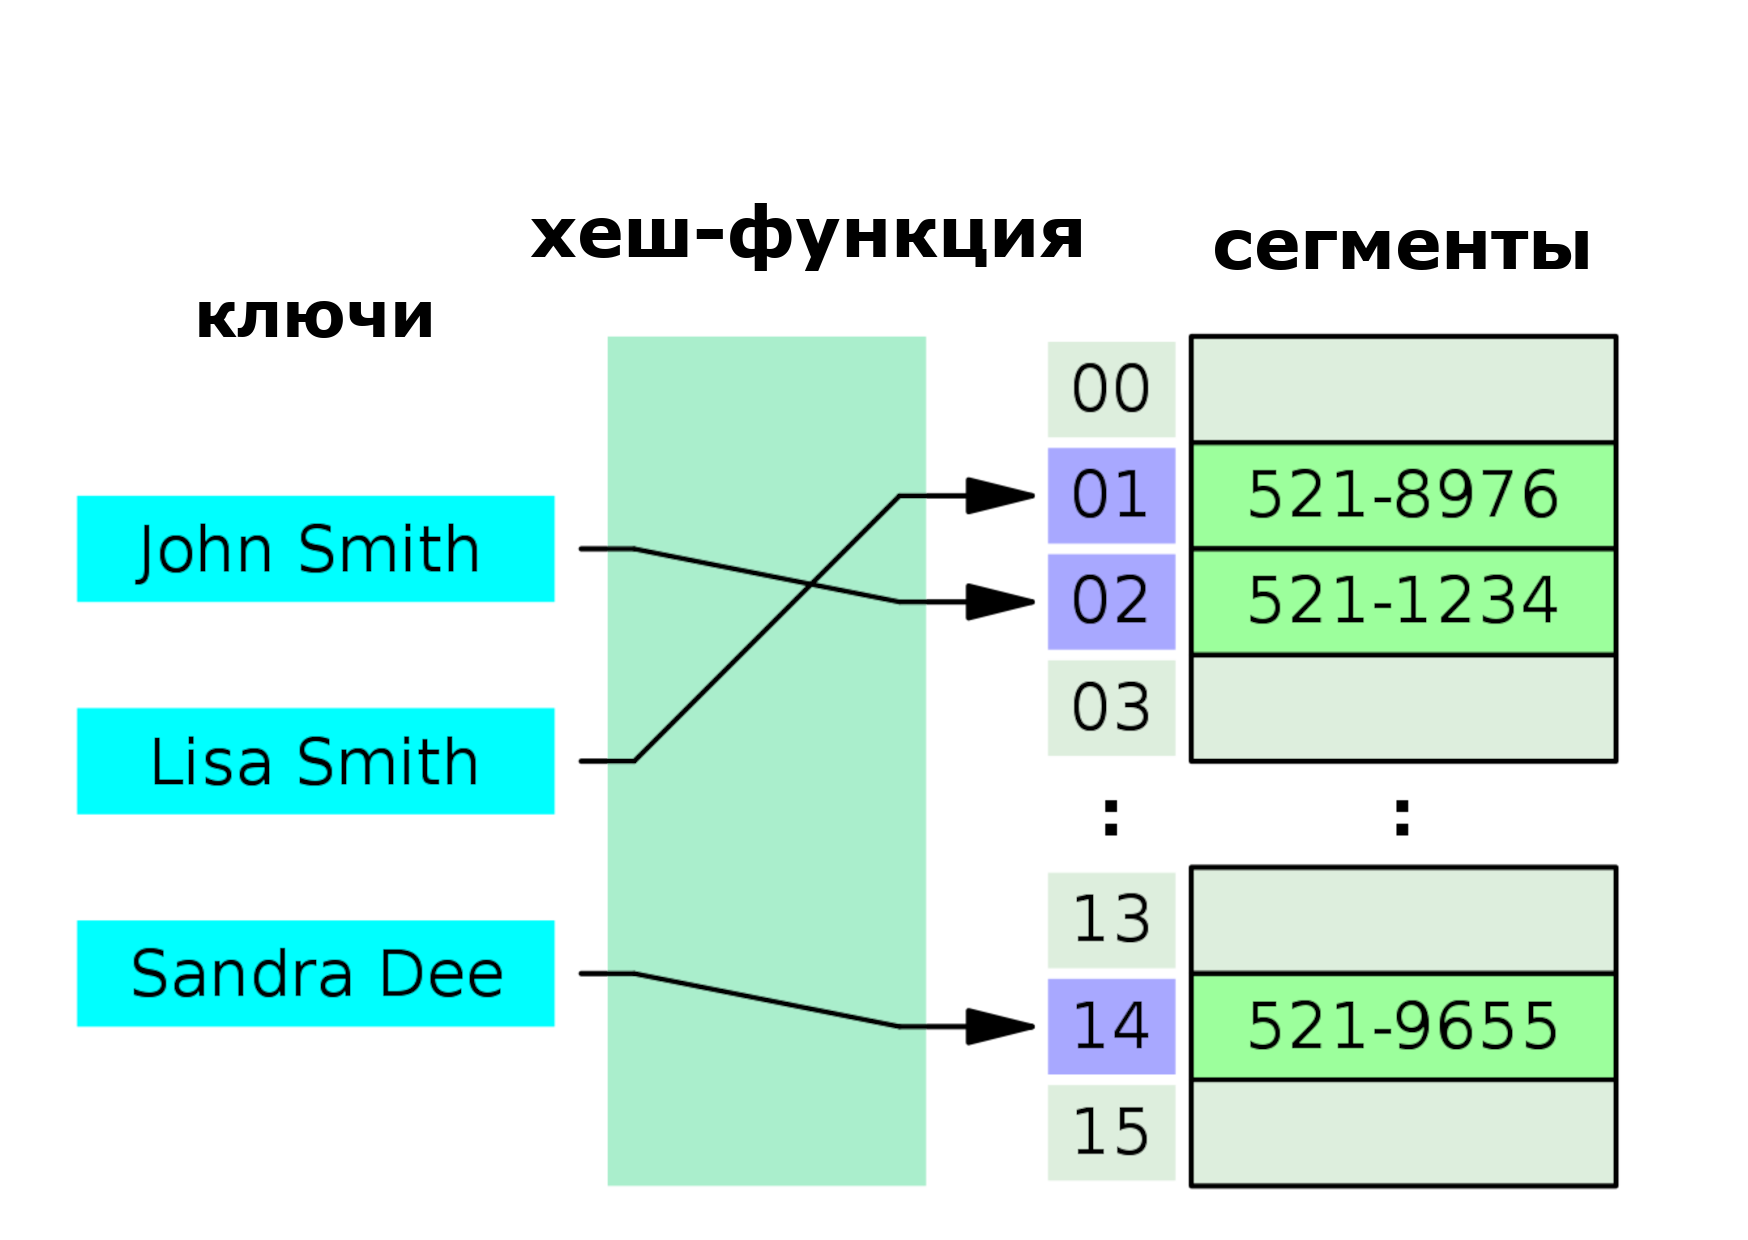
\includegraphics[scale=0.7]{phonebook.png}
		\caption{Небольшая телефонная книга в качестве хэш-таблицы}
	\end{center}
\end{figure}

\subsection{История}

Идея хеширования возникла независимо в разных местах.
В январе 1953 года Ханс Петер Лун написал внутренний меморандум IBM, в котором использовалось хеширование с методом цепочек (метод разрешения коллизий).
Джин Амдал, Элейн М. Макгроу, Натаниэль Рочестер и Артур Сэмюэль примерно в одно и то же время внедрили программу, использующую хеширование.
Открытая адресация (ещё один метод разрешения коллизий) с линейным проходом приписывается Амдалу, но у российского академика Андрея Ершова была та же идея.\cite{HansPeterLuhn}

\section{Хеширование}

Преимущество использования хеширования заключается в том, что адрес таблицы записи может быть вычислен непосредственно из ключа.
Хеширование подразумевает функцию $h$, которая при применении к ключу $k$ создает хэш $M$. 
Однако, поскольку $M$ может быть потенциально большим, результат хеша должен быть сопоставлен размеру таблицы.
Наиболее распространенным методом является метод деления, в котором при вычислении слота используется модульная арифметика.

\[h(k)=M \% N\]

Это часто делается в два этапа,

\[M = h(k)\]
\[i = M \% l\]

Где $i$ - адрес таблицы (индекс), а $l$ - размер таблицы.

В нашей работе мы использовали метод класса Object GetHashCode() для вычисления хешей объекта.
В C\# эта функция служит хеш-функцией по-умолчанию.
Все классы в C\# наследуются от Object, так что не составит труда вызвать данный метод.
Метод возвращает хеш-код для текущего объекта.

\section{Разрешение коллизий}

Алгоритм поиска, использующий хеширование, состоит из двух частей. 

Первая часть - это вычисление хэш-функции, которая преобразует ключ поиска в индекс таблицы. 
Идеальный случай таков, что никакие два ключа поиска не хэшируют один и тот же индекс таблицы, однако это не всегда так, и это невозможно исключить для невидимых заданных данных. 

Следовательно, вторая часть алгоритма - разрешение коллизий. 

Двумя распространенными методами разрешения коллизий являются метод цепочек и открытая адресация.

В нашей работе мы использовали цепочки.

\subsection{Метод цепочек}

Метод цепочек - это процесс, который включает в себя создание связанного списка с парой ключ-значение для каждого индекса поискового массива. 
Элементы, которые имеют коллизии объединены в единый связанный список, который можно просмотреть, чтобы получить доступ к элементу с помощью уникального ключа поиска. 
Разрешение коллизий с помощью цепочки, т.е. с помощью связанного списка, является распространенным методом реализации.

\begin{figure}[H]
	\begin{center}
		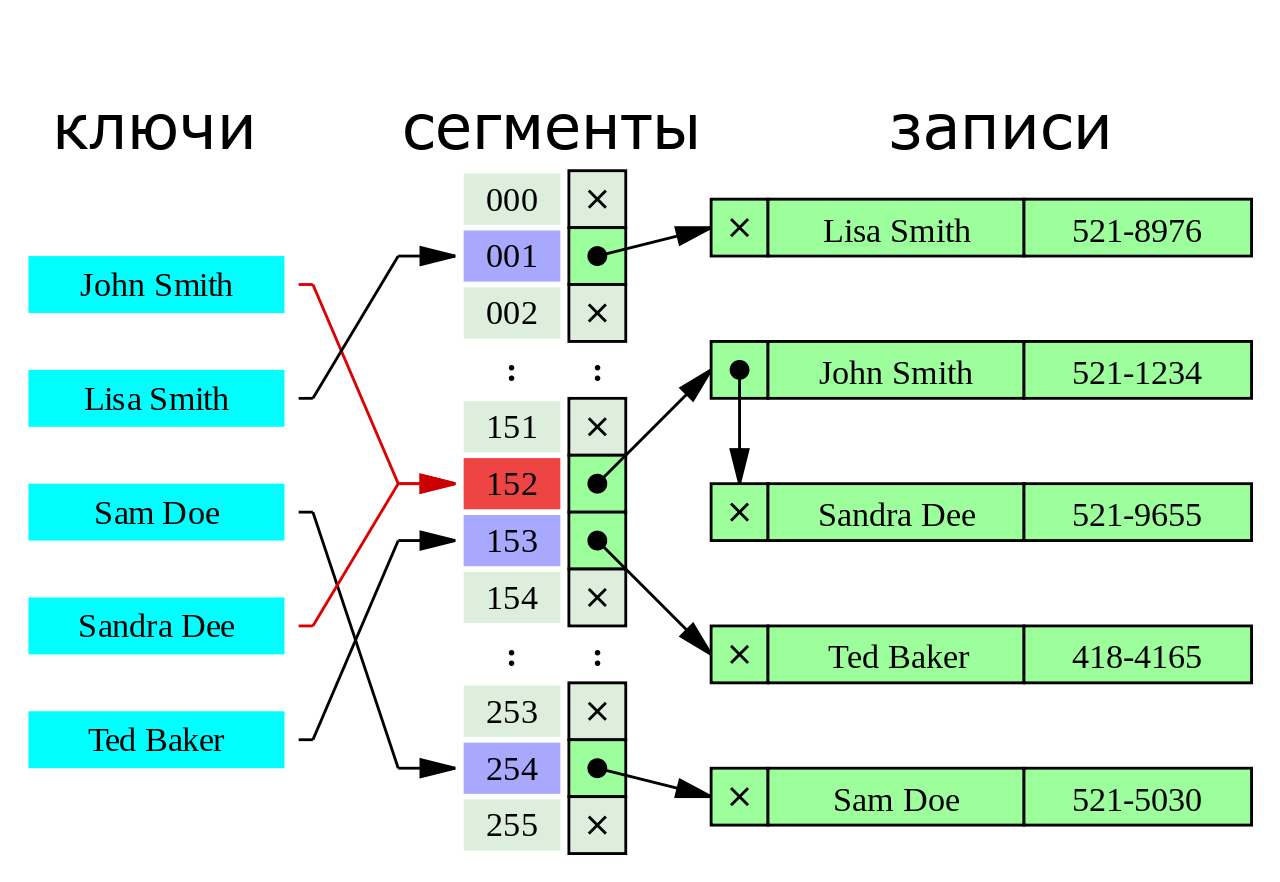
\includegraphics[width=\textwidth]{coll.png}
		\caption{Коллизия хешей разрешена с помощью метода цепочек}
	\end{center}
\end{figure}

\subsection{Метод открытой адресации}

В другой стратегии, называемой открытой адресацией, все записи ввода хранятся в самом массиве bucket.
Когда необходимо вставить новую запись, сегменты проверяются, начиная с хэшированного слота и продолжая в некоторой последовательности проверки, пока не появится найдено незанятое место.
При поиске записи сегменты сканируются в той же последовательности, пока либо не будет найдена целевая запись, либо не будет найден неиспользуемый слот массива, что указывает на то, что такого ключа в таблице нет.

\begin{figure}[H]
	\begin{center}
		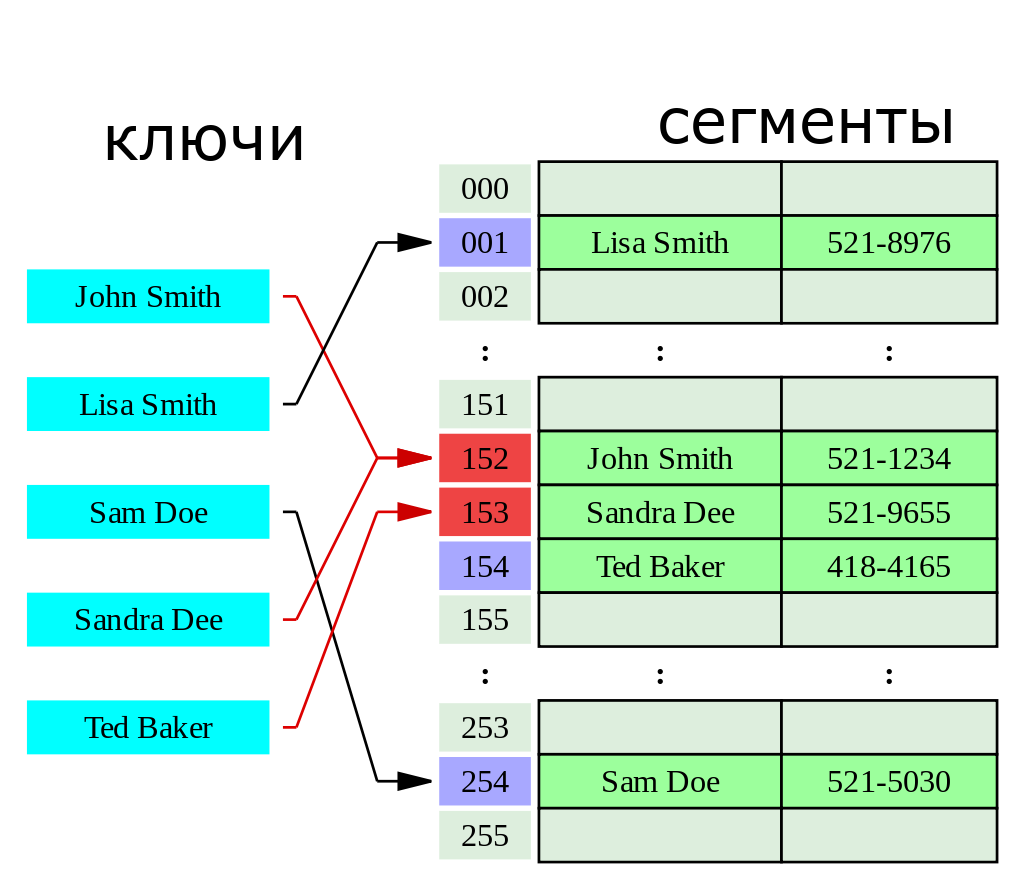
\includegraphics[width=\textwidth]{colloaddr.png}
		\caption{Коллизия хешей разрешена путем открытой адресации с линейным проходом (интервал =1). Обратите внимание, что "Ted Baker" имеет уникальный хэш, но, тем не менее, столкнулся с "Sandra Dee", которая ранее сталкивалась с "John Smith".}
	\end{center}
\end{figure}

\section{Используемые инструменты и технологии}

\begin{itemize}
	\item Git - система контроля версий. Разработка в команде невозможна без данной технологии. Весь код располагается на GitHub: \url{https://github.com/tstuteam/HashTable}.
	\item Windows - операционная система, на которой были произведены тесты.
	\item Visual Studio, Rider, Visual Studio Code - интегрированные среды разработки, а так же текстовые редакторы, с помощью которого был напечатан данный отчёт.
	\item WPF - аналог WinForms, система для построения клиентских приложений Windows с визуально привлекательными возможностями взаимодействия с пользователем, графическая (презентационная) подсистема в составе .NET Framework (начиная с версии 3.0), использующая язык XAML.
	\item XUnit - это удобный и самый современный фреймворк для модульного тестирования для C\#.
	\item \LaTeX - был использован для компиляции текста отчёта в данный документ, который вы читаете.
\end{itemize}

\section{Код библиотеки}

\begin{code}
	\lstinputlisting[language=Java]{../../Classes/HashTable.cs}
	\caption{HashTable.cs - Код библиотеки}
\end{code}

\newpage
\section*{Заключение}
Делаем заключение. Типа работу сделали, можно доделать то-то сё-то.
\addcontentsline{toc}{section}{Заключение}